%%
%% This is file `sample-sigplan.tex',
%% generated with the docstrip utility.
%%
%% The original source files were:
%%
%% samples.dtx  (with options: `sigplan')
%% 
%% IMPORTANT NOTICE:
%% 
%% For the copyright see the source file.
%% 
%% Any modified versions of this file must be renamed
%% with new filenames distinct from sample-sigplan.tex.
%% 
%% For distribution of the original source see the terms
%% for copying and modification in the file samples.dtx.
%% 
%% This generated file may be distributed as long as the
%% original source files, as listed above, are part of the
%% same distribution. (The sources need not necessarily be
%% in the same archive or directory.)
%%
%% The first command in your LaTeX source must be the \documentclass command.
\DocumentMetadata{
  lang=en,
  pdfversion=2.0,
  %pdfstandard=ua-2,
  %testphase={phase-III,firstaid,math,title}
  tagging=on,
  testphase={phase-III,firstaid,math,title}
  %tagging-setup={math/setup=mathml-SE}
}
\documentclass[sigplan,screen,nonacm]{acmart-tagged}
\usepackage{color}
\setlength {\marginparwidth }{2cm}
\usepackage[colorinlistoftodos]{todonotes}
\usepackage[
    type={CC},
    modifier={by-nc-sa},
    version={4.0},
]{doclicense}
%% NOTE that a single column version is required for 
%% submission and peer review. This can be done by changing
%% the \doucmentclass[...]{acmart} in this template to 
%% \documentclass[manuscript,screen,review]{acmart}
%% 
%% To ensure 100% compatibility, please check the white list of
%% approved LaTeX packages to be used with the Master Article Template at
%% https://www.acm.org/publications/taps/whitelist-of-latex-packages 
%% before creating your document. The white list page provides 
%% information on how to submit additional LaTeX packages for 
%% review and adoption.
%% Fonts used in the template cannot be substituted; margin 
%% adjustments are not allowed.
%%
%% \BibTeX command to typeset BibTeX logo in the docs
\AtBeginDocument{%
  \providecommand\BibTeX{{%
    \normalfont B\kern-0.5em{\scshape i\kern-0.25em b}\kern-0.8em\TeX}}}












%%
%% end of the preamble, start of the body of the document source.
\begin{document}

%%
%% The "title" command has an optional parameter,
%% allowing the author to define a "short title" to be used in page headers.
\title{Assessing Flaws in CAPTCHA Security through Progress in AI}

%%
%% The "author" command and its associated commands are used to define
%% the authors and their affiliations.
%% Of note is the shared affiliation of the first two authors, and the
%% "authornote" and "authornotemark" commands
%% used to denote shared contribution to the research.
\author{Jaydon A. Stanislowski}
\email{stani152@morris.umn.edu}
\affiliation{%
  \institution{Division of Science and Mathematics 
	\\
        University of Minnesota, Morris
	}
  \city{Morris}
  \state{Minnesota}
  \country{USA}
  \postcode{56267}
}

%%
%% By default, the full list of authors will be used in the page
%% headers. Often, this list is too long, and will overlap
%% other information printed in the page headers. This command allows
%% the author to define a more concise list
%% of authors' names for this purpose.
%\renewcommand{\shortauthors}{Trovato and Tobin, et al.}

%%
%% The abstract is a short summary of the work to be presented in the
%% article.
\begin{abstract}
Turing tests are widely employed on the Internet in the form of CAPTCHAs, short challenges designed to identify and prevent artificial web traffic. This technology is important for web security as a whole, and yet, as computational models become more sophisticated, its effectiveness only wanes. In this paper, we examine recent research on the growing threat to CAPTCHA security, in particular, the widely-used reCAPTCHA v2 and v3, and explore proposals to reinforce it against future attacks.
\end{abstract}

\doclicenseThis

%%
%% Keywords. The author(s) should pick words that accurately describe
%% the work being presented. Separate the keywords with commas.
\keywords{CAPTCHA, reCAPTCHA, Turing test, artificial intelligence, neural networks, reinforcement learning, internet, security}


%%
%% This command processes the author and affiliation and title
%% information and builds the first part of the formatted document.
\maketitle

\section{Introduction}
\label{sec:introduction}

CAPTCHA, short for "Completely Automated Public Turing test to tell Computers and Humans Apart," is one of the most widely used security tools on the modern Internet, created to help mitigate bot traffic on websites. Maintaining the reliability of such tools is essential, as they defend millions of websites from spam, web scraping, credential stuffing (a type of attack against user login info that involves automatically testing several common or recycled passwords), and fake users pretending to be human actors.

\begin{figure}[h]
\centering
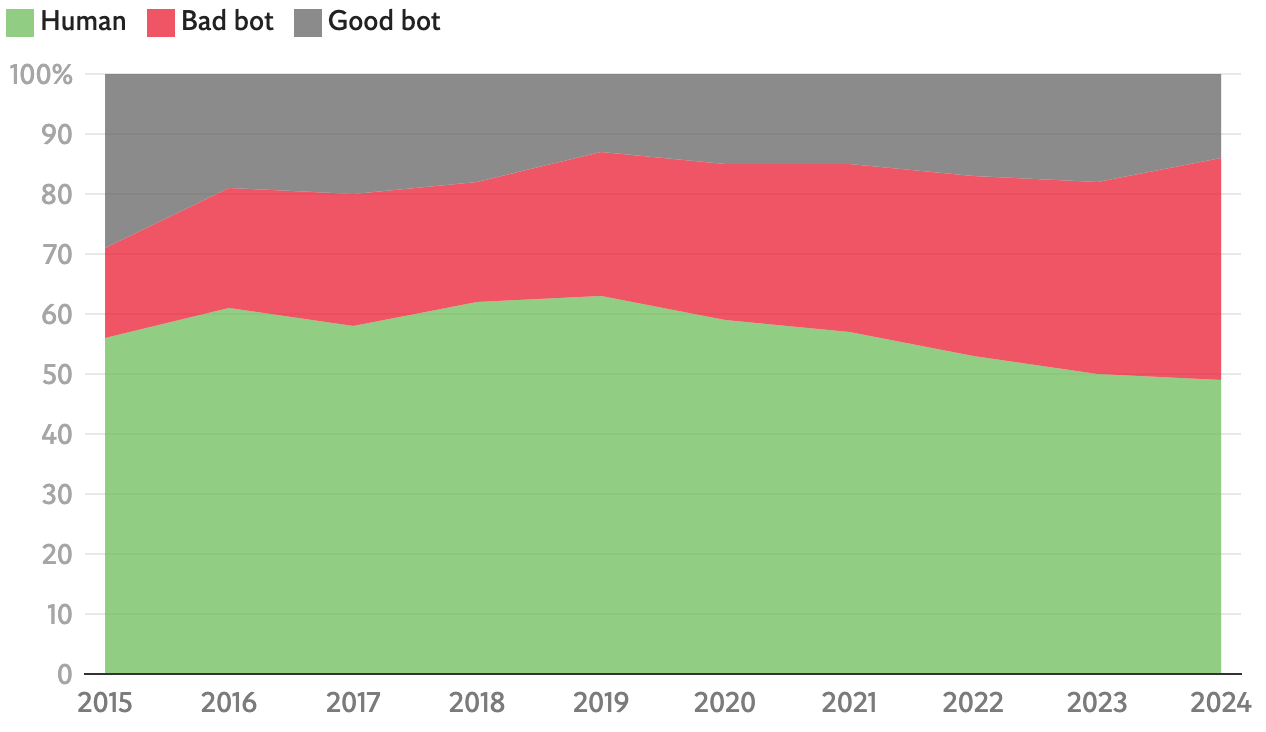
\includegraphics[width=1\linewidth]{resources/bots}
\caption{A graph of global internet traffic over recent years [1]}
\label{fig:bots}
\end{figure}

\todo[inline, color=pink]{I don't really know if there's a better way to cite this in-line. This graph comes from an article by The Independent, but the data itself is from the 2025 Imperva Bad Bot Report.}

In recent years, malicious artificial web traffic has increased substantially, with experts believing that bots accounted for over half of all web traffic in 2024, as shown in Figure \ref{fig:bots}. As AI technology has evolved over the years, so has the capacity for machines to simulate human intelligence, thereby bypassing security measures designed to impede them. AI models are now capable of performing a broad range of tasks previously thought to only be possible for humans to complete, further redefining what it takes to differentiate a computer from a real person. The increasingly sophisticated nature of these models poses a threat to the safety of the web as a whole, and yet, CAPTCHA development is seemingly unable to keep up.

This paper reviews the extent to which AI models are capable of bypassing modern CAPTCHA security, primarily focusing on the development of Google's reCAPTCHA as a case study. We will explain the computational models used in recent research to complete the tasks required by the most widely used CAPTCHAs today, and it will evaluate how successful the models are in this goal. The paper will also discuss predictions for how the threat to the Internet may grow with time, and explore recent proposals to improve existing tools to reinforce CAPTCHA security.
 

\section{Background}
\label{background}

\subsection{Origin of CAPTCHAs}
\label{sec:background-captcha}

The term CAPTCHA was first conceived by Luis von Ahn et al. [2] in the early 2000's to describe a form of Turing test for the purpose of preventing spam and bot attacks on the Internet. The Turing test was originally designed by Alan Turing to assess machine intelligence by evaluating its ability to mimic human intelligence [3]. In the Turing test, a human evaluator holds a conversation with a machine and a human simultaneously, with the goal of identifying which is the human and which is the machine. According to Turing, if the machine is able to fool the evaluator, then it demonstrates an ability to exhibit intelligence similar to that of a human.

A CAPTCHA is slightly different from a Turing test in that, rather than a human evaluator and two participants, the test is administered automatically by a machine and taken by a single participant who may be a human or a bot. According to Luis von Ahn et al., ``A CAPTCHA is a cryptographic protocol whose underlying hardness assumption is based on an AI problem'' [2]. In order for a CAPTCHA program to be effective, it must be able to grade and provide tests that cannot be passed by current AI models, but are easy for humans to solve. The developers of CAPTCHA believed that, if a CAPTCHA challenge is successfully broken by AI, it ``implies a win-win situation'' because ``a useful AI problem is solved,'' further advancing the field.

\begin{figure}[h]
\centering
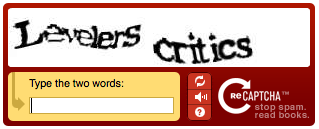
\includegraphics[width=1\linewidth]{resources/v1}
\caption{An example of a reCAPTCHA v1 challenge}
\label{fig:v1}
\end{figure}

Many such tests have been developed and used widely on the Internet over the past two decades. A well-known example is the first iteration of reCAPTCHA, known as reCAPTCHA v1. This type of CAPTCHA challenge is text-based, requiring the participant to transcribe a short string of text deemed difficult or impossible for machines to read, as shown in Figure \ref{fig:v1}. The text is often manipulated to further obscure from more sophisticated models, via warping, rotating, scaling, or the addition of random noise [4]. ReCAPTCHA v1 was deprecated in 2018, as the degree of complexity required to make it effective became too great, placing an unnecessary burden on human participants that defeated the purpose of CAPTCHA.

Since the development of these text-based CAPTCHAs, other types of challenges have dominated the web. In particular, the later versions of reCAPTCHA provide more sophisticated means of assessing participants while reducing friction for users. reCAPTCHA v2 and v3 simply "test" the participant by collecting hidden metrics about browser activity, discussed further in section \ref{sec:metrics}. If the participant is scored to be a potential risk, they may be asked to solve another challenge, such as an image labeling problem, described in section \ref{sec:visual}.

Today, CAPTCHA challenges that analyze browser data have largely replaced both text- and image-based CAPTCHAs, although many websites still use image labeling challenges as a complete alternative or a second check should a user fail the former challenge. Despite the seeming effectiveness of combining these challenges, they are independently quite insecure, as discussed in section \ref{sec:bypassing}.

\subsection{Artificial Intelligence}
\label{sec:background-ai}

In order to understand the role of artificial intelligence in CAPTCHA security, it is helpful to first examine the details of the tools involved in cracking it.

\subsubsection{Convolutional Neural Networks}
\label{sec:background-cnn}

These AI models are typically employ to solve computer vision problems, or problems that task computers with identifying and analyzing objects or text in images. Due to their increasing effectiveness in recent years thanks to hardware developments, they are, to some extent, able to be trained and run on normal computers, posing a risk to web security applications that identify bots via image labeling problems.

Regular neural networks are a type of computational model based on human neurons, designed to simulate how humans learn sophisticated concepts and form mental associations. They consist of interconnected layers of nodes, where numerical data is transmitted between each node and manipulated via some activation function, whose parameters are determined by weights that get adjusted through the learning process. CNNS are unique in that they typically take an image as input, and compute an output that classifies the image via hidden (intermediate) layers that perform processes known as convolution and pooling.

\todo[inline, color=pink]{Todo: Explain convolution and pooling in some detail, maybe just enough to span the rest of this page. This is still something that I'm very unfamiliar with—maybe having an extra meeting just to discuss and explain this would help.}


\subsubsection{Reinforcement Learning}
\label{sec:background-rl}

\todo[inline, color=pink]{I haven't done sufficient research on reinforcement learning to write much here, but it is definitely a priority.}


\section{Modern reCAPTCHA Challenges}
\label{sec:modern-captchas}

\todo[inline, color=pink]{Somewhere here, I need to include something about how reCAPTCHA was acquired by Google for clarity, though I'm not sure where to slot that in.}

As mentioned in section \ref{sec:background-captcha}, modern versions of reCAPTCHA, namely, v2 and v3, primarily depend on collecting user metrics to assess the risk of bot activity, while also providing an image labeling challenge in alternative cases. This section will first discuss in detail how the image labeling challenges are created and served to the user, then touch on what is known about the metric-based challenges, according to existing research.

\subsection{Image Labeling}
\label{sec:visual}

\todo[inline, color=pink]{This section will mainly focus on reCAPTCHA v2.}

\subsection{Behavioral Metrics}
\label{sec:metrics}

Google's reCAPTCHA v2, first implemented in 2013, was the first tool to introduce an "invisible" CAPTCHA, a type of verification challenge that did not explicitly ask the user to solve a challenge to measure intelligence, but purely operated in the background and scored users based on browsing habits. This has been expanded on with reCAPTCHA v3, released in 2017. The tool regularly collects data as the user browses the web, returning a score ranging from 0 (highly likely to be a bot) to 1 (likely a human). While this type of challenge has been praised for reducing tedium resulting from CAPTCHA challenges for real users, many have criticized it for intruding on user privacy [5]. \todo[inline, color=pink]{Not sure how relevant this last sentence is, or where to include it.} 

\begin{figure}[h]
\centering
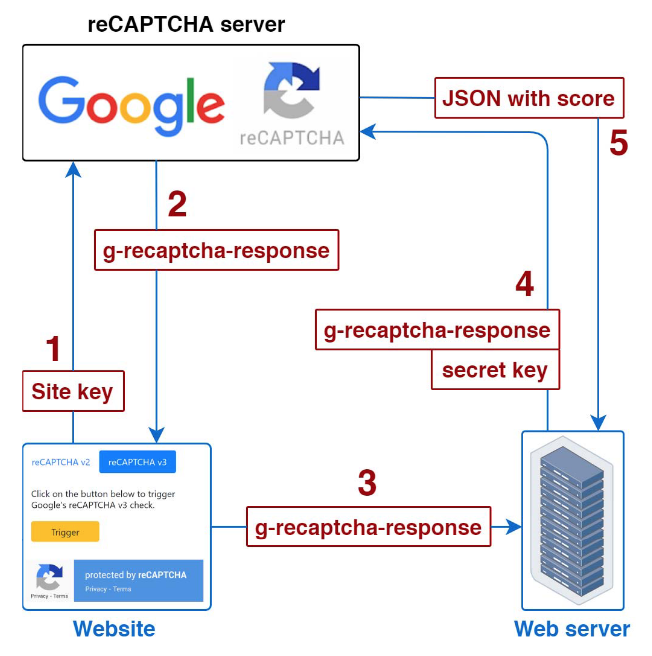
\includegraphics[width=0.7\linewidth]{resources/v3-workflow}
\caption{reCAPTCHA v3 verification workflow, adapted from [6]}
\label{fig:v3}
\end{figure}

ReCAPTCHA v3 differs from v2's "invisible" challenge in that the user is never asked to check a box, but rather, it collects user data over time, and verification occurs either when the user clicks a button on a website that is bound to v3, or automatically invoked through some other action taken by the user. This verification is done through generating an encrypted token on the website's back end that contains the necessary metrics. This token is then sent to Google's servers, which return a response containing the user's score, whereupon the website can programmatically decide which actions to take. Figure \ref{fig:v3} illustrates this process in detail [6].

Since reCAPTCHA v3 is proprietary, not much is known about exactly which metrics the tool collects, or how they contribute to the overall score. Additionally, keeping this information confidential is important to protecting the security of the software, as knowledge of it could theoretically be used to engineer a perfectly undetectable bot. However, Tsingenopoulos et al. [6] identified, through analysis of some source code, 

\section{Breaking reCAPTCHA}
\label{sec:bypassing}

\subsection{reCAPTCHA v2 and CNNs}
\label{sec:v2}

\subsection{reCAPTCHA v3 and RL}
\label{sec:v3}

\section{Proposals to Improve CAPTCHAs}

\section{Conclusion}


\begin{acks}
I sincerely thank Dr. Elena Machkasova for her invaluable work in not only instructing the fall 2025 senior seminar course, but also guiding me through the writing process and helping me stay motivated during this challenging semester. I also thank the University of Minnesota Morris for providing me the opportunity to conduct this literature review and present my work to my peers.
\end{acks}

%%
%% The next two lines define the bibliography style to be used, and
%% the bibliography file.
\bibliographystyle{ACM-Reference-Format}
\bibliography{sources}


\end{document}
\endinput
%%
%% End of file `sample-sigplan.tex'.